
%
%  $Description: Author guidelines and sample document in LaTeX 2.09$
%
%  $Author: ienne $
%  $Date: 1995/09/15 15:20:59 $
%  $Revision: 1.4 $
%

\documentclass[times, 10pt,twocolumn]{article}
\usepackage{latex8}
\usepackage{times}
\usepackage{hyperref}
\usepackage{graphicx}

%\documentstyle[times,art10,twocolumn,latex8]{article}

%-------------------------------------------------------------------------
% take the % away on next line to produce the final camera-ready version
% \pagestyle{empty}

%-------------------------------------------------------------------------
\begin{document}

\title{MORA - A Sensor Data Analysis Toolkit for Mobile Phones}

\author{Heinrich Hartmann\\
University Koblenz\\ % WeST \\ % IN-F
% Ecublens, 1015 Lausanne, Switzerland\\ Paolo.Ienne@di.epfl.ch\\
% For a paper whose authors are all at the same institution,
% omit the following lines up until the closing ``}''.
% Additional authors and addresses can be added with ``\and'',
% just like the second author.
\and
Christoph Schaefer \\
University Koblenz \\
% First line of institution2 address\\ Second line of institution2 address\\
% SecondAuthor@institution2.com\\
\and
Matthias Thimm \\
University Koblenz \\
}

\maketitle
\thispagestyle{empty}

\begin{abstract}
\end{abstract}

%-------------------------------------------------------------------------
\Section{Introduction} %% MT
- Much sensor data from smartphones available.

- Problem: Extract sensible information from raw data. E.g. for
  - Quantified Self
  - Internet of Things

- Need tools for gathering test data and evaluation of algorithms: MORA.

%-------------------------------------------------------------------------
\Section{MORA Toolkit}

The MORA toolkit provides a simple mean to record, transfer, store and
analyze sensor data from Android mobile phones. In the following
sections we given an overview about the overall architecture and
discuss the design choices of the individual components.

\SubSection{Overview}

Design goals of the MORA toolkit:
\begin{itemize}
\item Simple codebase. New developers should be able to contribute easily.
\item Low CPU usage on the mobile device (Battery efficiency, and allow high frequency recordings).
\item Data visualization and export tools included, to enable data mining and analysis in later steps.
\item Privacy awareness. Give the users control over their data.
\item Provide plugin interface e.g. for mobile data mining.
\item Reuse of existing standards and technologies. JSON. Postgres. NodeJS.
\end{itemize}

The Toolkit consists of three components:
\begin{itemize}
\item \textbf{Mobile Sensor Collector}.  Records great varity of
  sensors. Flexible event loop/dispatcher - design. Essentially single
  threaded. Plugins storage, bulk transfer and streaming built-in.
\item \textbf{Sensor Storage Service}.
  Receives data over HTTP or ZeroMQ, inserts into Database and File System.
\item \textbf{Data Inspection Service}.  Gives convenient view on data
  stored in database. Allows users to keep control over their data.
\end{itemize}

Flexible serialization format {\bf Json Sensor Format}.


* How are the goals achieved?

\begin{figure}[h]
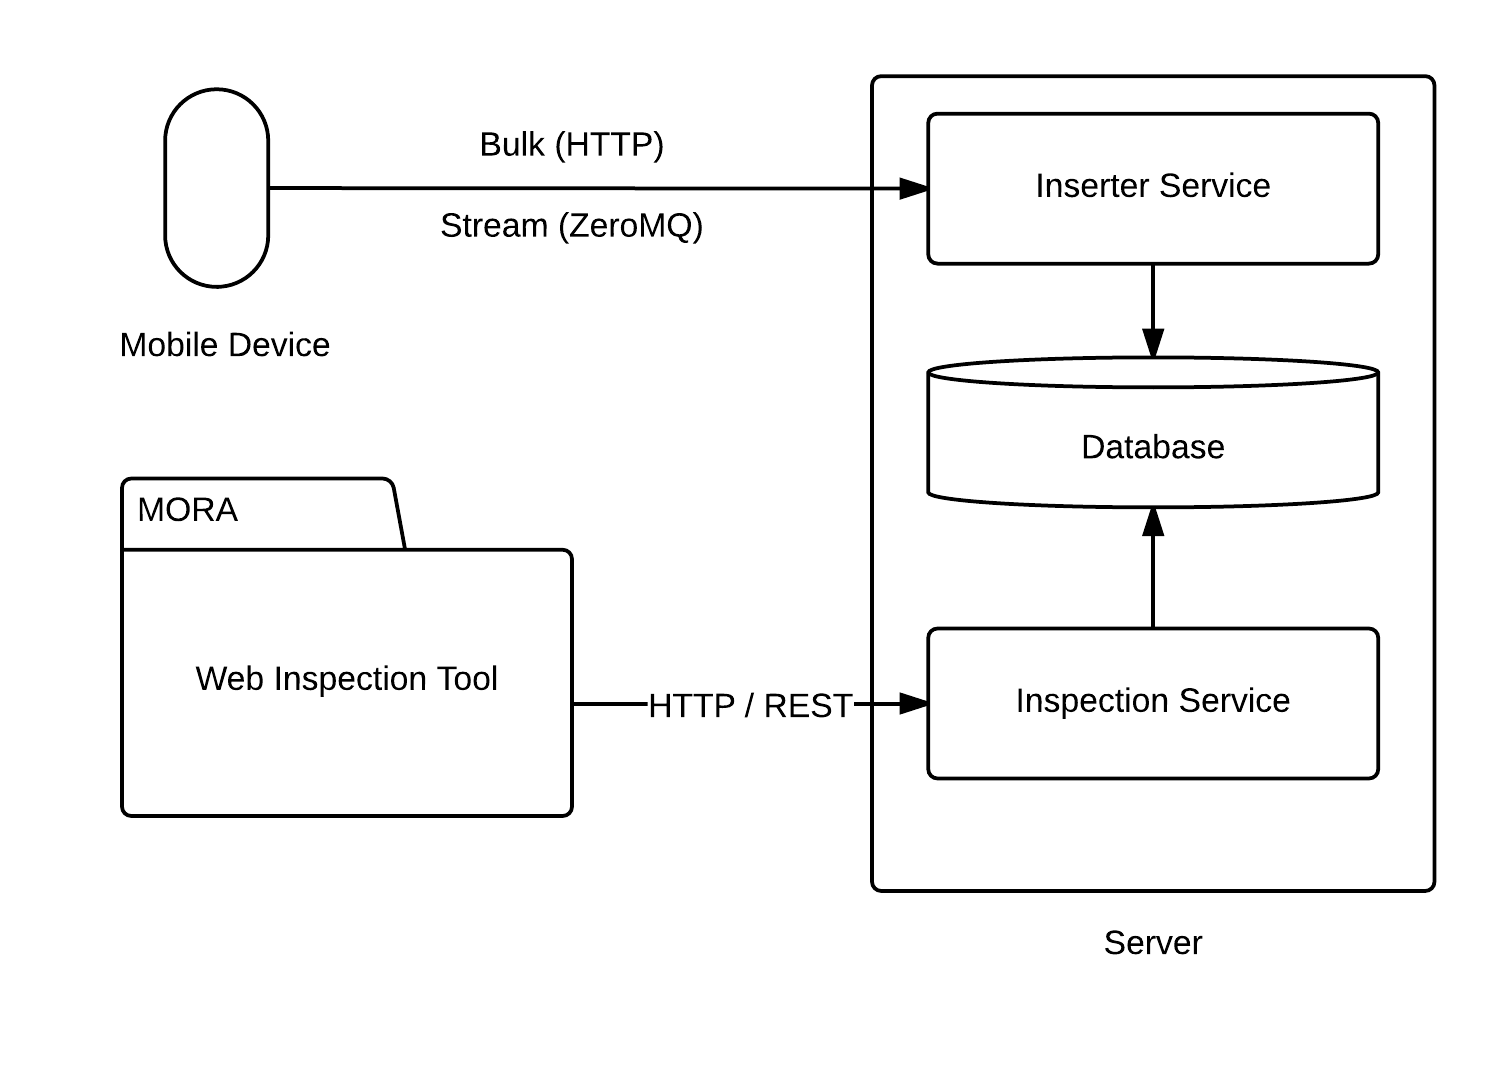
\includegraphics[width=\linewidth]{img/system_overview.png}
\caption{MORA System Overview}
\label{overview}
\end{figure}

\SubSection{Mobile Sensor Collector}

\begin{figure}[h]
\begin{center}
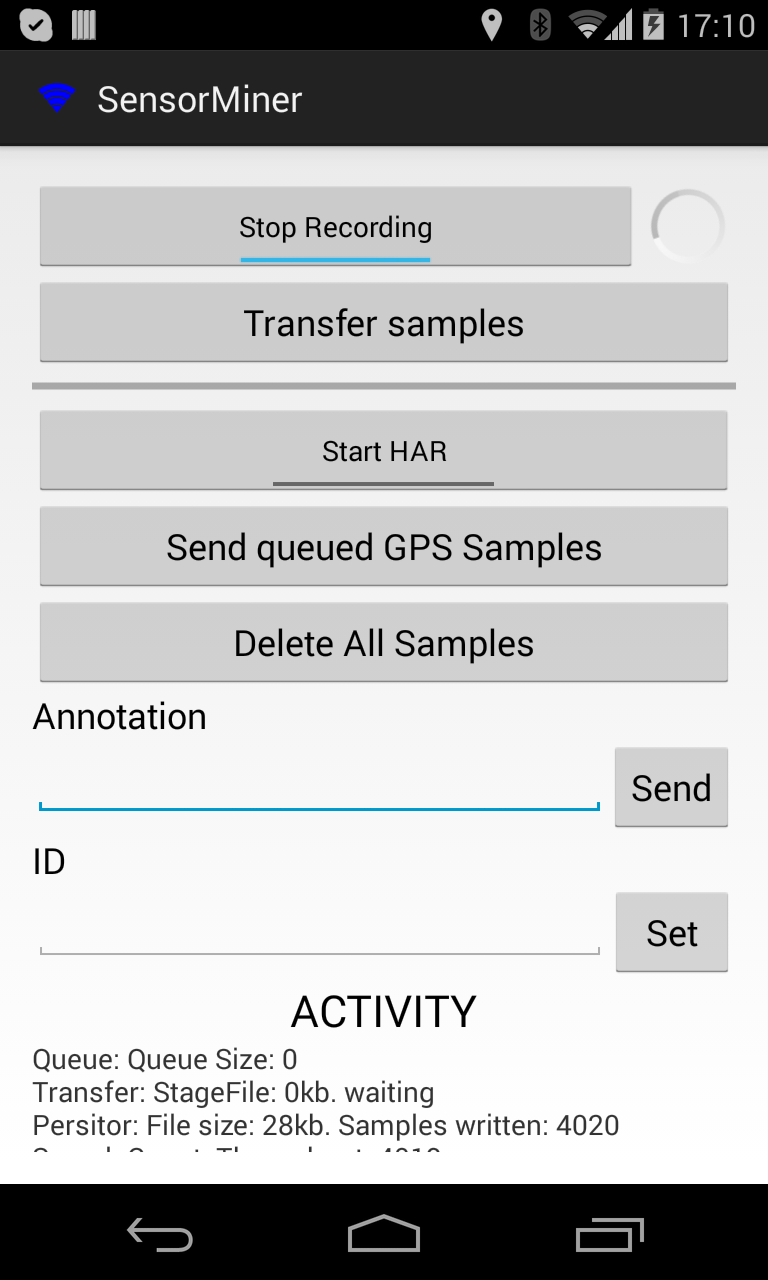
\includegraphics[width=3cm]{img/sc_gui.png}
\end{center}
% TODO: Replace by Lukas new GUI
\caption{Mobile Sensor Collector GUI}
\label{mobile}
\end{figure}


\begin{figure}[h]
\begin{center}
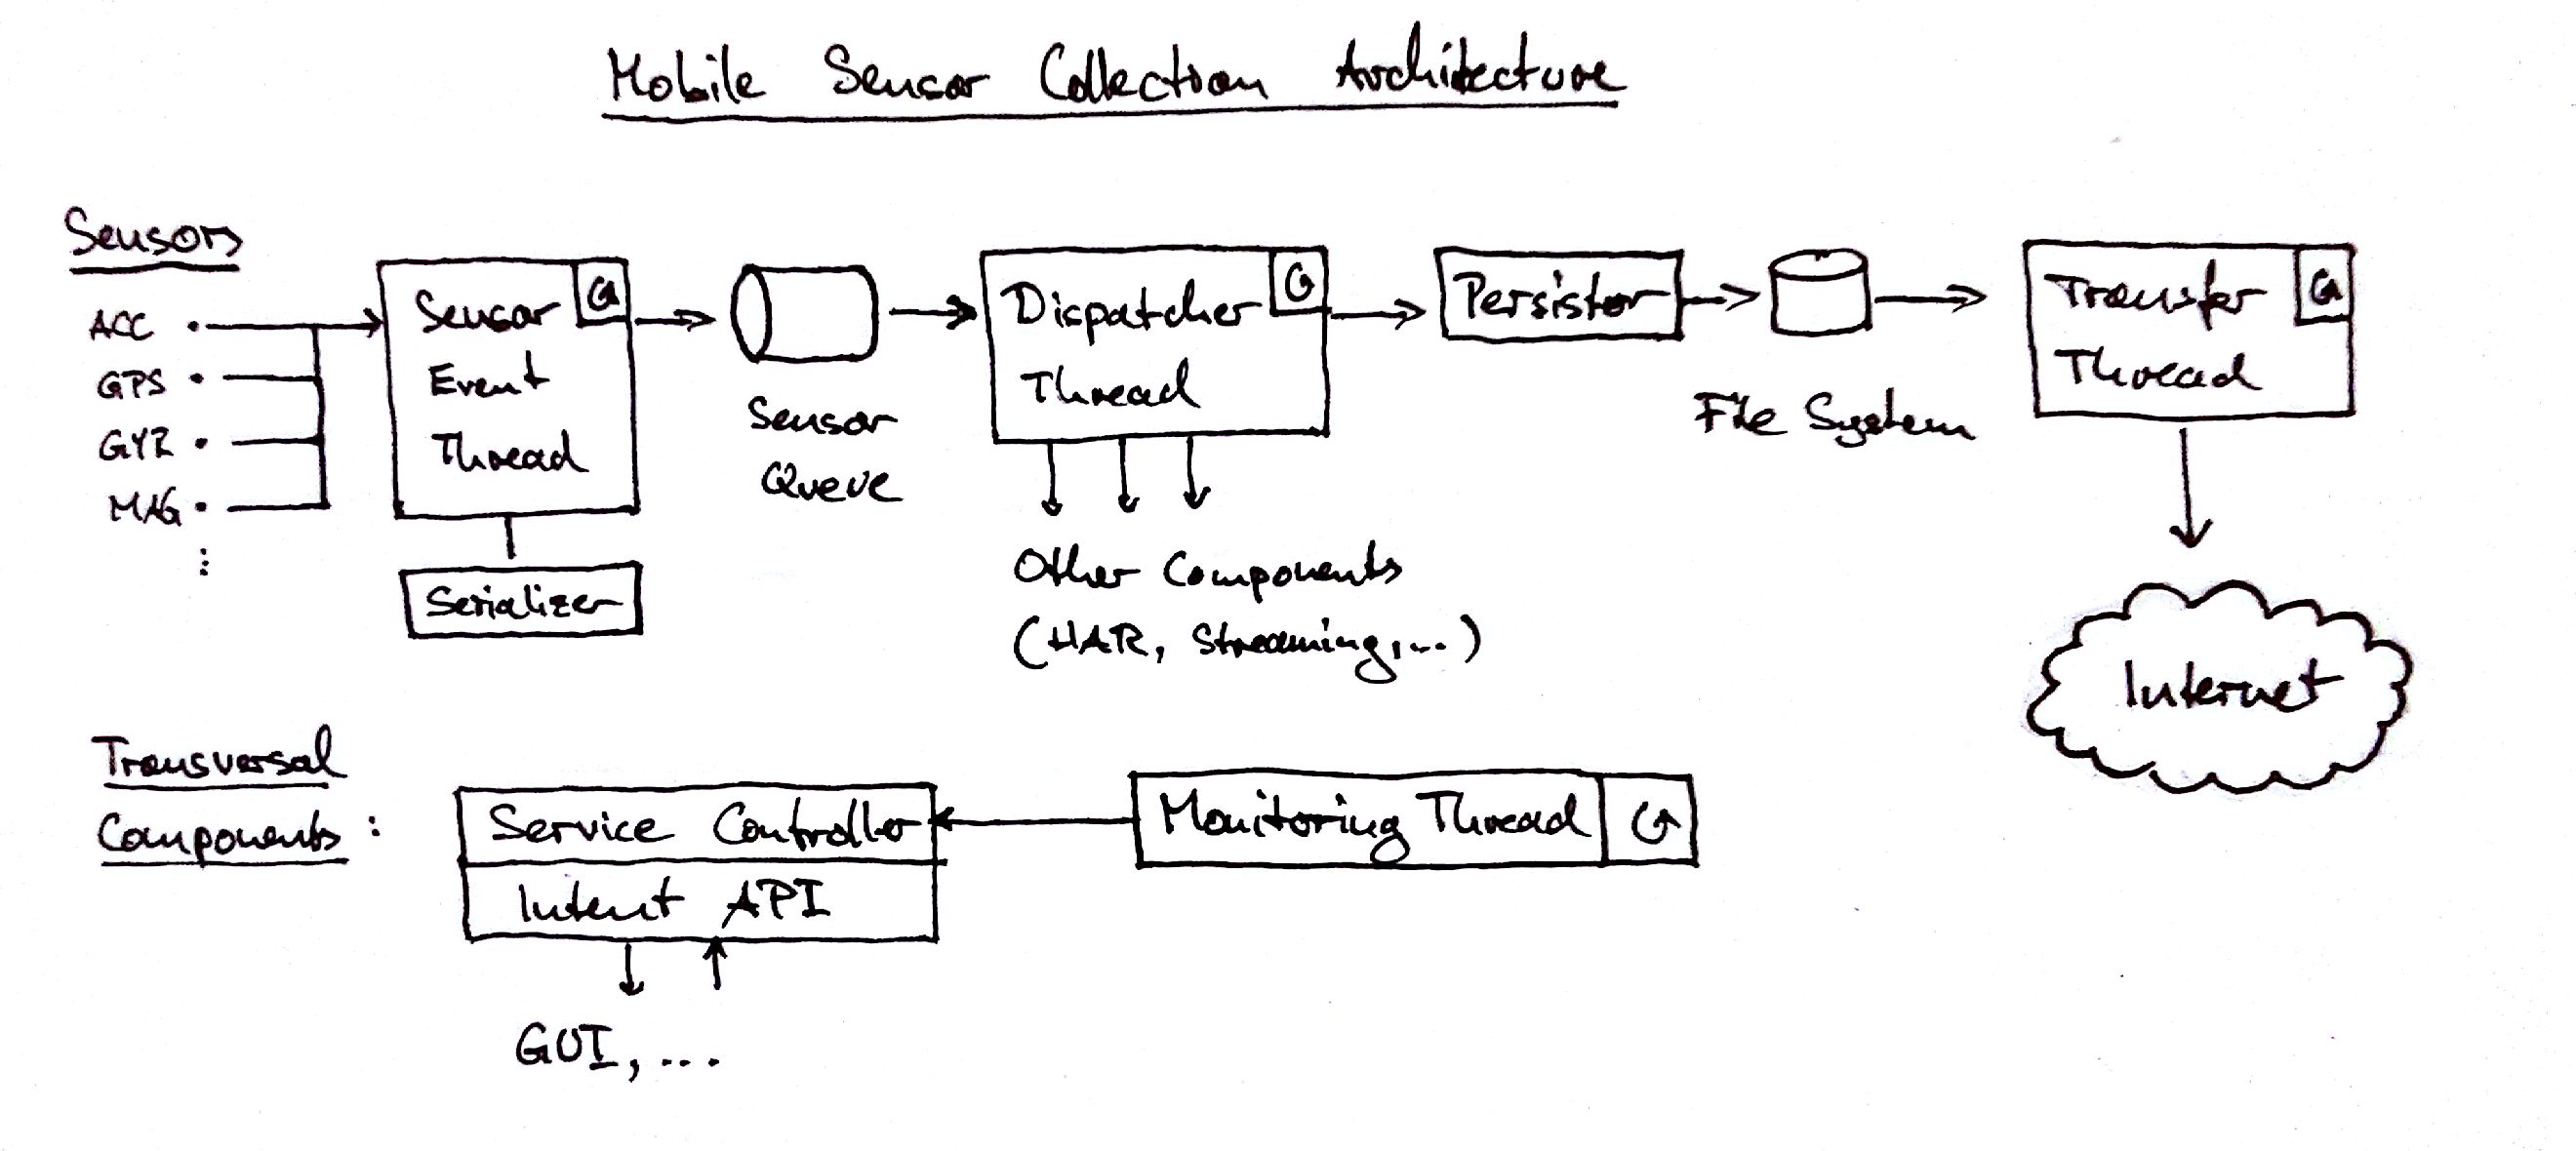
\includegraphics[width=\linewidth]{img/sc_architecture.jpg}
\end{center}
% TODO: Replace by Lukas new GUI
\caption{Mobile Sensor Collector Architecture}
\label{mobile}
\end{figure}

* Goals and 'Requirements'
  - Correctness of data / good performance
  - View sensor data as events, that are logged / streamed / processed
  - Extensible by analysis plugins
  - Transfer of sensor data to server

* Service + Example GUI (Communication with Intent bindings)
  - Android lifecycle forces collector to be a service
  - Standalone use of service possible and intended

* Available Sensors. Types of sensors. Class Hierarchy.

* Data flow from Sensor Event to Log file,
  in analogy to logging frameworks.
  Use of Threads

* Transfer via HTTP and Streaming

* Configuration options with configuration file and GUI

* Log messages are written to a file

* Extendability with Plugins: Consumer/Producer. Examples:
  - HAR
  - GPS Cache
  - Intent producer

\SubSection{Sensor Storage Server}

* HTTP server (tomcat/Node), that accepts POST request

* Stores in FS and in DB

* Sends 200 Status code if insert in db complete

* JSF Data Exchange Format

* Auto Creation of DB Tables for new sample types (JSON data type)

\SubSection{Web Inspection Tool}

% http://liveandgov.uni-koblenz.de/storage/inspection

+ Figure: Screenshot mit Bar-Code Anzeige von Activities


An important step that should be considered before any data mining task is a manual data exploration phase. For this purpose, MORA provides a powerful data inspection tool. Using the web-based front end, a first overview of the data integrity can be obtained quickly. Both raw data and mining results can be viewed in the browser. Occasionally appearing transmission errors caused by the interaction of mobile phones and the back end, can be discovered easily by the user. In addition, plots for all sensor types give a rough measure for the quality of the recorded data. With the help of this presentation we could, for example, discover GPS inaccuracies or frequency deviations.

Besides time series plots and map based views of GPS data the inspection tool offers a bar-code-like representation (Figure~\ref{fig:inspectionBarcode}) which is able to display a large number of tags on a time axis.
To get more details all views can be zoomed in and out. On each zoom level the corresponding data of the displayed interval can be exported and downloaded as CSV (Figure~\ref{fig:inspectionRawData}).

\begin{figure}[h]
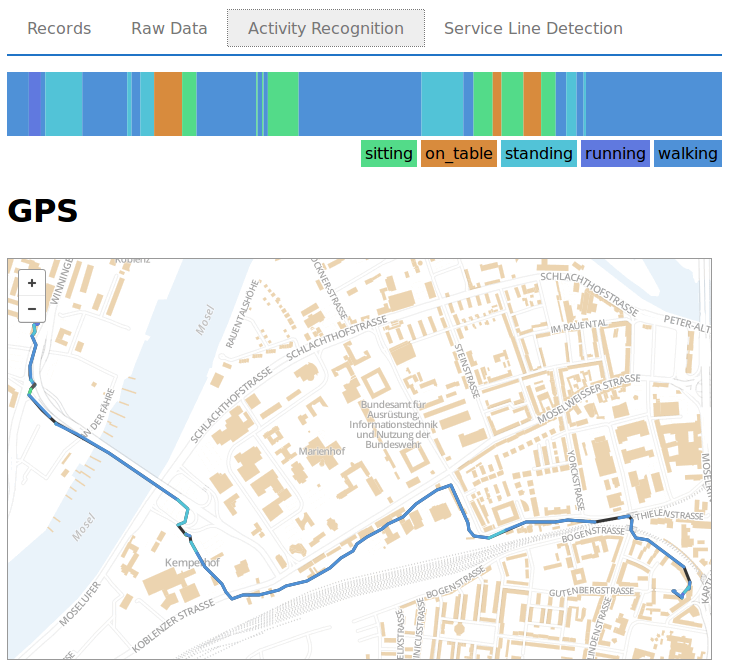
\includegraphics[width=\linewidth]{img/BarcodeScreenshot.png}
\caption{Bar-code-like representation of human activities in the inspection front end.}
\label{fig:inspectionBarcode}
\end{figure}
\begin{figure}[h]
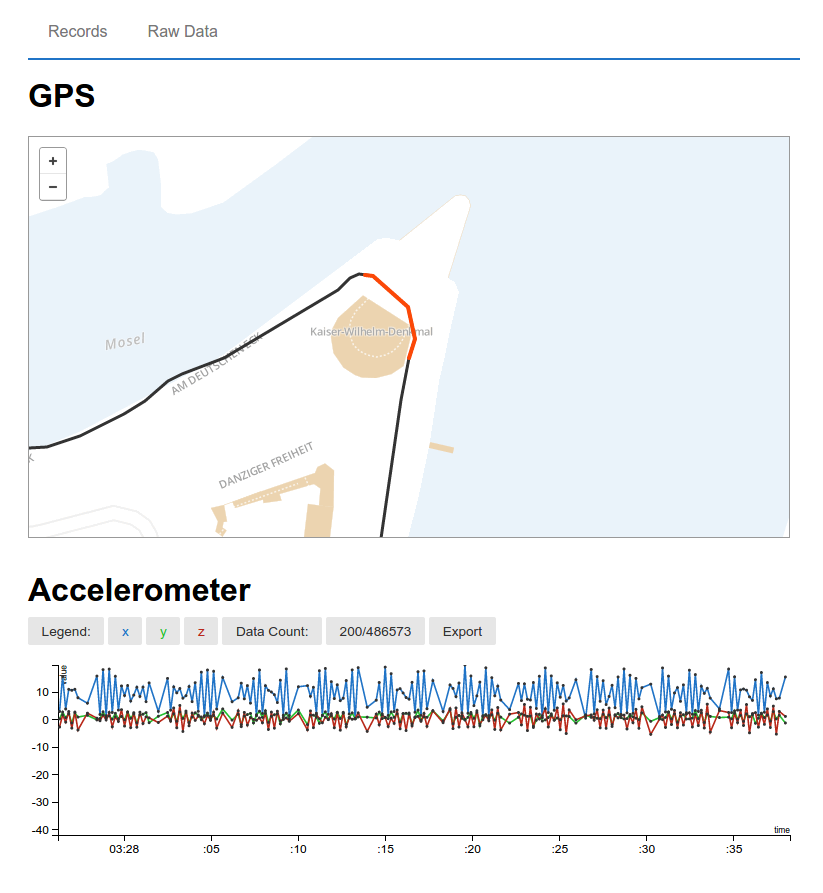
\includegraphics[width=\linewidth]{img/InspectionTool_RAW.png}
\caption{Zoomed in map view and the corresponding accelerometer raw data in the inspection front end.}
\label{fig:inspectionRawData}
\end{figure}

Via the web interface, all users have access to their recorded data and are entitled to delete their tracks if necessary. Apart from the possibility to carry out small maintenance tasks, this give users the control over their data and thus enhances the privacy.



  - Automatic display of available tables
    - as text (TEXT) or plot (float)

* Mining output has to be stored in db
  - Can be created on mobile device and inserted into transfer file
  - Or can be done on the server

%-------------------------------------------------------------------------
\Section{Practical Examples}

\SubSection{Human Activity Recognition}
* Decision tree learning with WEKA
* Import classifier as JAVA class into MORA Library

\SubSection{Service Line Detection}
* Web service for SLD
* GPS Samples are gathered via MORA lib
* Query results are inserted back into MORA
* Analysis of classification results via inspection tool

%-------------------------------------------------------------------------
\Section{Related Work}

* FUNF
* SDCF


\nocite{ex1,ex2}
\bibliographystyle{latex8}
\bibliography{latex8}

\end{document}
